% Project paper: IEEE conference format, 4 pages.
% Build: pdflatex main && bibtex main && pdflatex main && pdflatex main
% (or upload the paper/ folder to Overleaf). The numbers in the results come
% from paper/generated/*.tex, which `python main.py train` writes; never type
% results in by hand.
\documentclass[conference]{IEEEtran}
\usepackage[T1]{fontenc}
\usepackage{graphicx}
\usepackage{booktabs}
\usepackage{amsmath}
\usepackage{cite}
\usepackage{xcolor}
\usepackage[hidelinks]{hyperref}
\graphicspath{{figures/}}

% Results macros (\BestModel, \BestMacroFOne, ...) produced by the pipeline
\newcommand{\BestModel}{Random Forest + class bias}
\newcommand{\BestMacroFOne}{0.8814}
\newcommand{\BestAccuracy}{0.9260}
\newcommand{\DetectionRate}{91.10\%}
\newcommand{\FalsePositiveRate}{6.492\%}
\newcommand{\NumRawFlows}{8,284,195}
\newcommand{\NumSampleFlows}{1,406,762}
\newcommand{\NumFeaturesIn}{78}
\newcommand{\NumFeaturesOut}{40}
\newcommand{\DataSourceNote}{}
\newcommand{\AEDetectionRate}{3.73\%}
\newcommand{\AEFalsePositiveRate}{1.01\%}
\newcommand{\AEAUC}{0.8705}

% Marks text the team must finish after the real run; set to {} for submission check
\newcommand{\fillin}[1]{\textcolor{red}{[#1]}}

\begin{document}

\title{Detecting Network Intrusions in CSE-CIC-IDS2018 with Rebalanced Tree Ensembles, Neural Networks and a Benign-Only Autoencoder}

\author{\IEEEauthorblockN{Student Name One}
\IEEEauthorblockA{MSCS 640\\ email@university.edu}
\and
\IEEEauthorblockN{Student Name Two}
\IEEEauthorblockA{MSCS 640\\ email@university.edu}}

\maketitle

\begin{abstract}
Signature-based defences miss novel attacks, and on flow data the attacks a
SOC cares about are rare. We build an end-to-end pipeline for 15-class
intrusion detection on CSE-CIC-IDS2018~\cite{sharafaldin2018}. It streams
\NumRawFlows{} raw flows in chunks, removes non-finite values, repeated headers,
duplicates and label-ambiguous flows, and builds a class-capped sample of
\NumSampleFlows{} flows. Feature selection reduces \NumFeaturesIn{} flow
statistics to \NumFeaturesOut{}. Class imbalance is handled on the training
split only, by Benign under-sampling, SMOTE~\cite{chawla2002} and damped class
weights. We compare a Random Forest baseline, gradient-boosted trees, an MLP
and their soft-voting ensemble, then tune per-class decision weights on
validation macro-$F_1$. The selected model, \BestModel{}, reaches a test
macro-$F_1$ of \BestMacroFOne{} and detects \DetectionRate{} of attack flows at a
false-positive rate of \FalsePositiveRate{}. A benign-only autoencoder adds
label-free anomaly scores for previously unseen attacks. The trained model is
served through a web dashboard that turns an uploaded CSV into a triaged
threat report.
\end{abstract}

\begin{IEEEkeywords}
intrusion detection, class imbalance, SMOTE, gradient boosting, autoencoder, CSE-CIC-IDS2018
\end{IEEEkeywords}

% ---------------------------------------------------------------------------
\section{Introduction}
Machine-learning network intrusion detection systems (NIDS) learn attack
behaviour from flow statistics rather than payload signatures. CSE-CIC-IDS2018
is a widely used benchmark for them~\cite{leevy2020}. Two properties make it
harder than headline accuracies suggest. First, it is severely imbalanced:
Benign flows outnumber the rarest attack, SQL Injection, by about five orders
of magnitude, so accuracy rewards a model that ignores attacks. Second, the
released CSVs contain labelling and processing artefacts, documented for the
closely related CIC-IDS2017~\cite{engelen2021} and for both
datasets~\cite{liu2022}. We therefore optimise and report \emph{macro}-$F_1$,
in which every class counts equally, and treat data engineering as a
first-class part of the method.

Our contributions are: (i) a memory-bounded, two-pass data pipeline for the
full 6.4\,GB dataset; (ii) a controlled comparison of tree ensembles and an
MLP under the same rebalancing; (iii) validation-tuned class-bias weights,
which raise macro-$F_1$ without touching the test set; and (iv) a deployed
dashboard that pairs the supervised classifier with an unsupervised anomaly
score.

% ---------------------------------------------------------------------------
\section{Dataset and Data Engineering}
\subsection{Data}
The ten ``Processed Traffic Data for ML Algorithms'' files contain one
CICFlowMeter record per bidirectional flow: 79 columns plus the
\texttt{Label}, and one day (20-02-2018) adds \texttt{Flow ID},
\texttt{Src IP}, \texttt{Src Port} and \texttt{Dst IP}. Each day has Benign
traffic plus only the attacks staged that day, so the training set is drawn
across all days. Table~\ref{tab:data} lists the classes, using the dataset's
own spellings.

\begin{table}[t]
\caption{Class distribution: all flows vs.\ the cleaned, capped sample}
\label{tab:data}
\centering\footnotesize
\begin{tabular}{lrr}
\toprule
Class & All flows & Clean sample \\
\midrule
Benign & 238,037 & 199,373 \\
Infilteration & 93,063 & 74,943 \\
\bottomrule
\end{tabular}

\end{table}

\subsection{Cleaning}
Reading proceeds in chunks of 250k rows, so no file is ever fully loaded.
Every chunk is cleaned as follows. (a) Header lines repeated mid-file are
removed. (b) Identifier and time columns (\texttt{Timestamp}, IPs, source
port, flow ID) are dropped: they describe the testbed rather than the
behaviour of the flow, and a model that used them would learn which host
attacked on which day. (c) All features are coerced to numbers.
\texttt{Infinity} and \texttt{NaN}, which appear in \texttt{Flow Byts/s} and
\texttt{Flow Pkts/s} when a flow has zero duration, become missing values and
are later imputed with the training median. Values outside the
\texttt{float32} range are clipped. (d) After sampling, exact duplicates are
removed, along with every copy of a feature vector that carries more than one
label, because no model can separate such flows and they only add label
noise.

\subsection{Sampling}
A first pass reads only the \texttt{Label} column and counts every class. A
second pass keeps each row with probability $\min(1, c/n_y)$, where $n_y$ is
the class count and $c$ is a cap (1M for Benign, 200k for each attack). Rare
classes are therefore kept in full, and the sample fits in laptop memory. The
de-duplicated sample is split 70/15/15 into stratified train, validation and
test sets. The validation set is used for early stopping, model selection and
decision tuning; the test set is used exactly once.

\subsection{Feature selection}
All selection is fitted on the training split. Each feature is median-imputed,
clipped to its $[10^{-4}, 1-10^{-4}]$ training quantiles, transformed with
$\operatorname{sign}(x)\log(1+|x|)$, which tames the heavy-tailed byte, rate
and duration features, and standardised. We then (1) drop zero-variance
columns (several bulk-rate and URG/PSH columns are constant), (2) rank
features with a class-balanced Extremely Randomized Trees
model~\cite{geurts2006} and, within every group whose pairwise $|r|>0.98$,
keep only the highest-ranked feature, and (3) keep the top 40. Fig.~\ref{fig:imp}
shows the resulting importances. \fillin{Comment on the top features once the
real run has finished, e.g.\ which packet-length, window-size or IAT features
dominate, and why that makes sense for DoS and brute-force traffic.}

\begin{figure}[t]
\centering
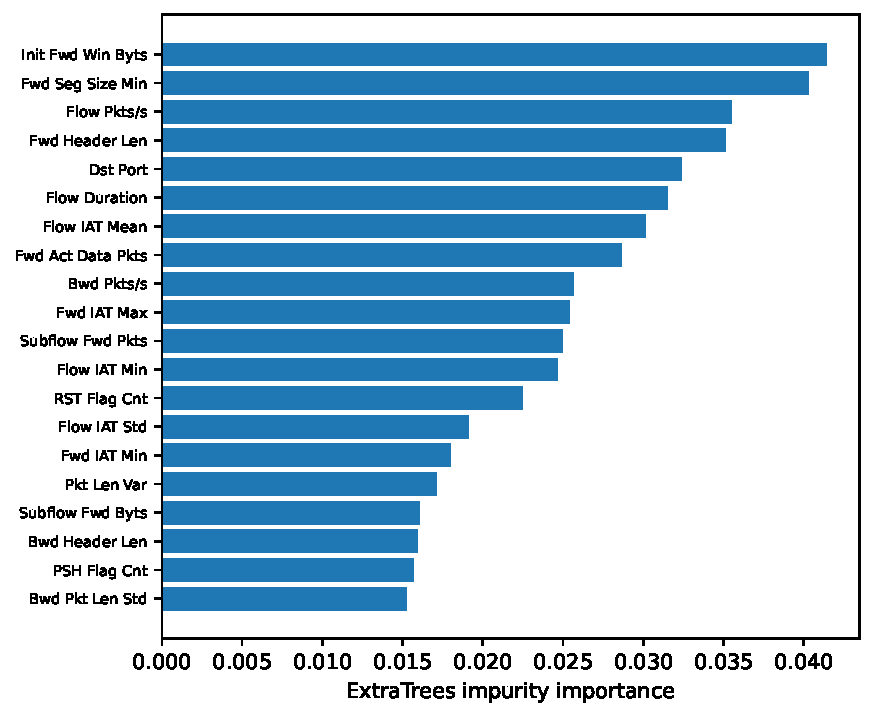
\includegraphics[width=0.92\columnwidth]{feature_importance}
\caption{Top-20 selected features by ExtraTrees impurity importance (training split).}
\label{fig:imp}
\end{figure}

\subsection{Class imbalance}
Imbalance handling is applied to the training split only, so the validation
and test sets keep the natural class mix. Benign is under-sampled to 600k
flows. Every class below 20k flows is lifted to 20k with
SMOTE~\cite{chawla2002}, which interpolates between a flow and one of its
$k{=}5$ nearest same-class neighbours in the standardised log space. All
models are trained with class weights $w_c=(n_{\max}/n_c)^{0.5}$, normalised
to a mean of 1. The exponent $0.5$ is a deliberate damping: once SMOTE has
lifted the rare classes, full inverse-frequency weighting costs Benign
precision, and with it the false-positive rate that an analyst actually
experiences.

% ---------------------------------------------------------------------------
\section{Models and Methodology}
\textbf{Random Forest} (baseline)~\cite{breiman2001}: 100 trees,
$\sqrt{d}$ features per split, 25\% bootstrap samples, depth $\le 25$, at
least 3 samples per leaf (a deliberate cap on model size and memory).
\textbf{Gradient-boosted trees}: XGBoost~\cite{chen2016} with histogram split
finding when it is available, otherwise scikit-learn's histogram GBDT, which
uses the same LightGBM-style binning~\cite{ke2017}. Learning rate 0.1, depth
8, L2 penalty 1, and up to 600 rounds with early stopping on validation log
loss. \textbf{MLP}: three ReLU layers (256-128-64), Adam~\cite{kingma2015},
batch size 1024, L2 penalty $10^{-4}$, early stopping, and the class weights
above applied to the cross-entropy loss. \textbf{Ensemble}: the average of the
three models' class probabilities. All models use
scikit-learn~\cite{pedregosa2011}.

\textbf{Class-bias decision rule.} The arg-max of the posterior is optimal
for accuracy, not for macro-$F_1$. For each model we learn non-negative weights
$\mathbf{w}$ and predict $\arg\max_c w_c\,p(c\mid x)$. The weights are found
by coordinate ascent over a log-spaced grid that maximises
\emph{validation} macro-$F_1$. Model selection likewise compares validation
macro-$F_1$ only.

\textbf{Hyper-parameter tuning.} \texttt{python main.py train --tune} runs a
random search (12 trials) over the GBDT learning rate, depth, leaf count and L2
penalty on a 150k-flow subsample, scored by validation macro-$F_1$. The
defaults above follow common practice for tabular data. \fillin{Report the
search outcome from \texttt{reports/results.json} (``tuning'') if you ran it.}

\textbf{Autoencoder.} A 32-8-32 bottleneck network is trained to reconstruct
Benign training flows only. A flow is flagged when its reconstruction error
exceeds the 99th percentile of errors on Benign validation flows. The
autoencoder never sees an attack label, so it complements the classifier on
attack types missing from training.

% ---------------------------------------------------------------------------
\section{Results}
Table~\ref{tab:models} compares the models; the $\star$ marks the model chosen
on validation. $F_1^M$ is macro-$F_1$ and $F_1^W$ is support-weighted $F_1$.
Table~\ref{tab:perclass} and Fig.~\ref{fig:cm} break down the selected model
by class, and Fig.~\ref{fig:roc} shows one-vs-rest and binary ROC curves.
Over all attack types combined, \BestModel{} detects \DetectionRate{} of
attack flows at a Benign false-positive rate of \FalsePositiveRate{}. The
autoencoder alone reaches an attack-vs-benign AUC of \AEAUC{}, flagging
\AEDetectionRate{} of attacks at \AEFalsePositiveRate{} false positives.

\begin{table}[t]
\caption{Model comparison (validation and held-out test)}
\label{tab:models}
\centering\footnotesize\setlength{\tabcolsep}{3.2pt}
\resizebox{\columnwidth}{!}{\begin{tabular}{lccccr}
\toprule
Model & Val $F_1^{M}$ & Test $F_1^{M}$ & Test $F_1^{W}$ & Test Acc. & Train (s) \\
\midrule
Random Forest & 0.8174 & 0.8138 & 0.9270 & 0.9255 & 23 \\
XGBoost & 0.8495 & 0.8338 & 0.9258 & 0.9225 & 584 \\
MLP & 0.7888 & 0.7766 & 0.9185 & 0.9176 & 2691 \\
Soft-vote ensemble & 0.8480 & 0.8259 & 0.9278 & 0.9270 & 3298 \\
Random Forest + class bias $\star$ & 0.8948 & 0.8814 & 0.9274 & 0.9260 & 23 \\
XGBoost + class bias & 0.8632 & 0.8532 & 0.9261 & 0.9228 & 584 \\
MLP + class bias & 0.8408 & 0.8366 & 0.9209 & 0.9261 & 2691 \\
Soft-vote ensemble + class bias & 0.8891 & 0.8499 & 0.9284 & 0.9302 & 3298 \\
\bottomrule
\end{tabular}
}
\end{table}

\begin{table}[t]
\caption{Per-class test results of the selected model}
\label{tab:perclass}
\centering\footnotesize
\begin{tabular}{lcccr}
\toprule
Class & Prec. & Rec. & $F_1$ & Support \\
\midrule
Benign & 0.946 & 0.935 & 0.941 & 132,086 \\
Bot & 1.000 & 0.998 & 0.999 & 15,171 \\
Brute Force -Web & 0.455 & 0.866 & 0.597 & 82 \\
Brute Force -XSS & 0.970 & 0.941 & 0.955 & 34 \\
DDOS attack-HOIC & 1.000 & 0.999 & 1.000 & 11,431 \\
DDOS attack-LOIC-UDP & 1.000 & 1.000 & 1.000 & 259 \\
DoS attacks-GoldenEye & 1.000 & 0.999 & 1.000 & 6,209 \\
DoS attacks-Hulk & 1.000 & 1.000 & 1.000 & 12,544 \\
DoS attacks-SlowHTTPTest & 0.833 & 1.000 & 0.909 & 5 \\
DoS attacks-Slowloris & 0.998 & 0.998 & 0.998 & 1,457 \\
FTP-BruteForce & 1.000 & 0.500 & 0.667 & 4 \\
Infilteration & 0.556 & 0.604 & 0.579 & 17,615 \\
SQL Injection & 0.727 & 0.667 & 0.696 & 12 \\
SSH-Bruteforce & 1.000 & 1.000 & 1.000 & 14,106 \\
\bottomrule
\end{tabular}

\end{table}

\begin{figure}[t]
\centering
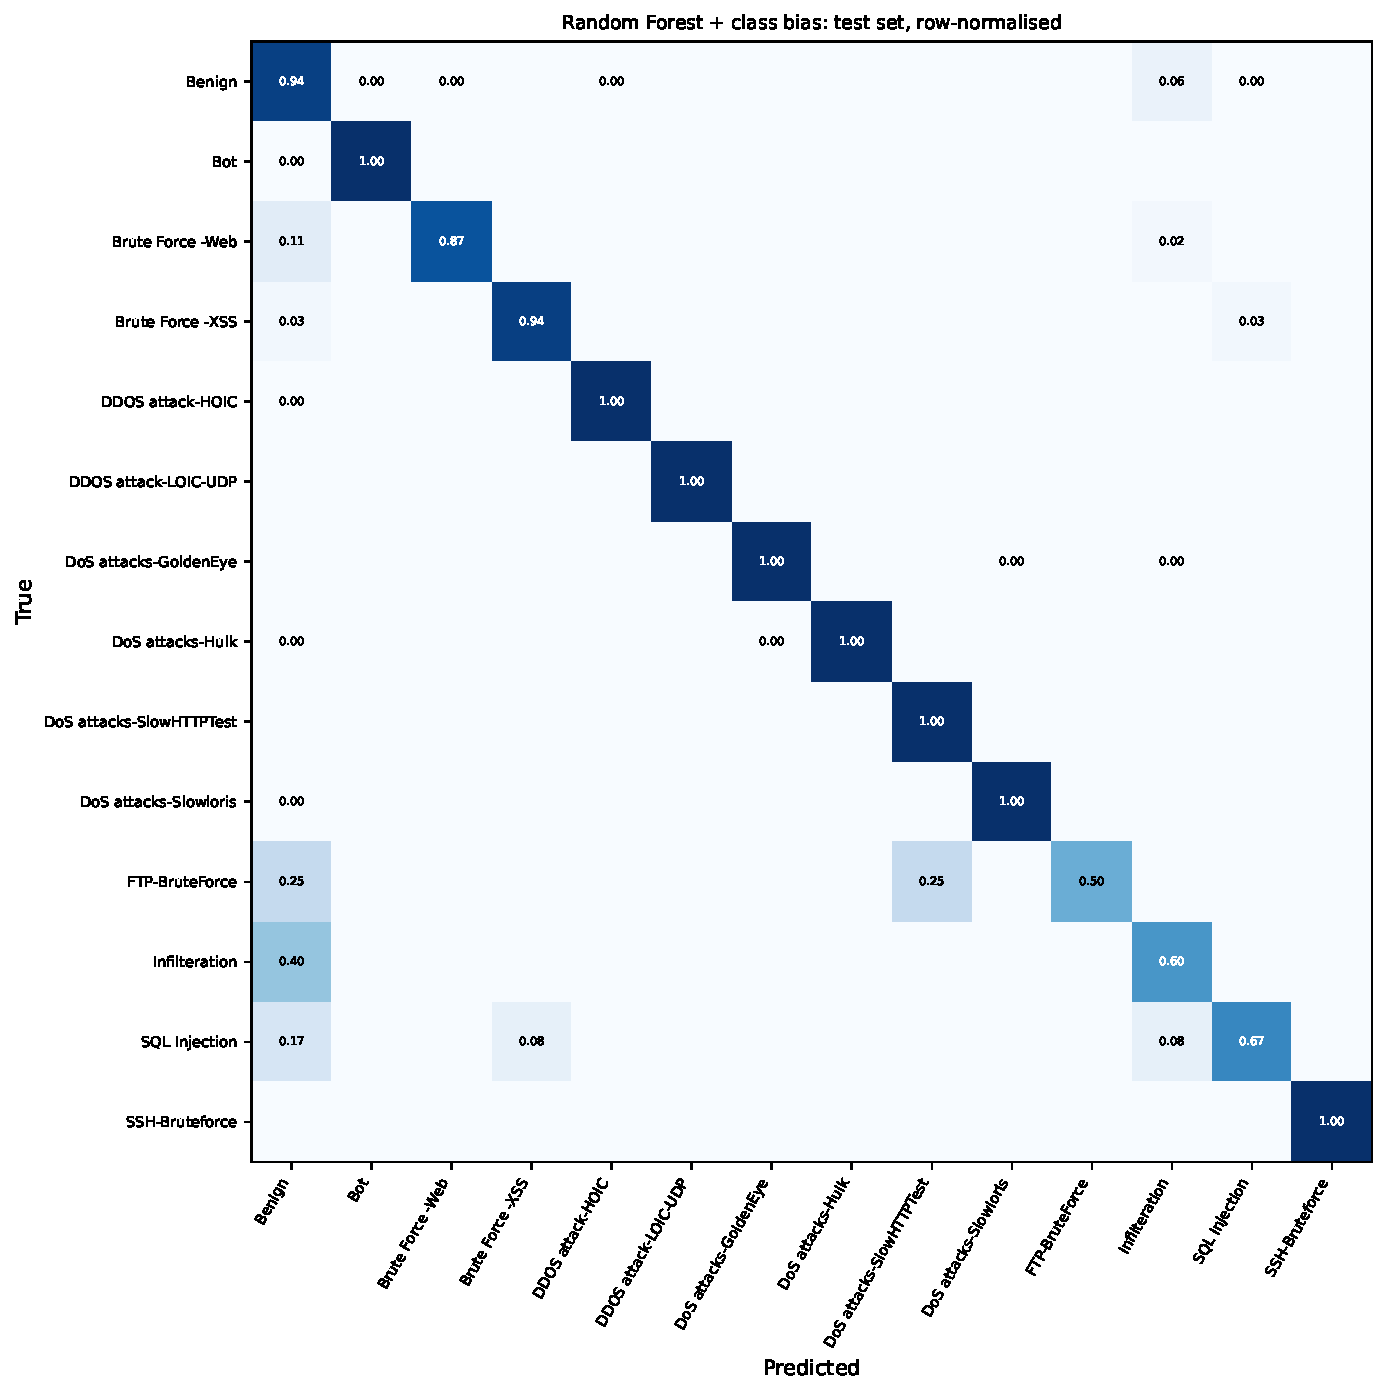
\includegraphics[width=\columnwidth]{confusion_matrix}
\caption{Row-normalised test confusion matrix of the selected model.}
\label{fig:cm}
\end{figure}

\begin{figure*}[t]
\centering
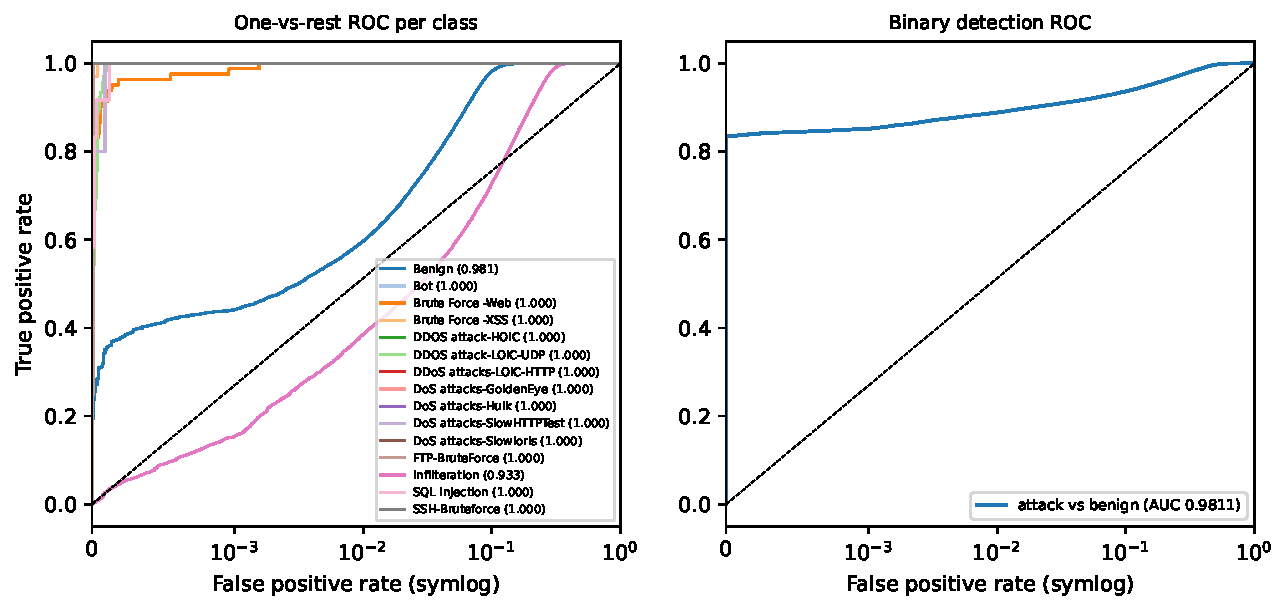
\includegraphics[width=0.82\textwidth]{roc_curves}
\caption{Test ROC curves (log-scaled FPR): one-vs-rest per class (left) and attack-vs-benign (right).}
\label{fig:roc}
\end{figure*}

\fillin{Discussion, written from the real numbers: (1) which model wins and by
how much over the RF baseline; (2) how much the class-bias step adds; (3)
the confusions. Prior analyses of this dataset lead us to expect
\emph{Infilteration} to be largely indistinguishable from Benign at the flow
level, and \emph{Brute Force -Web}, \emph{Brute Force -XSS} and \emph{SQL
Injection} to be confused with each other because they share a target and a
traffic shape; check whether Fig.~\ref{fig:cm} confirms this before you state it.}

% ---------------------------------------------------------------------------
\section{Deployment}
\texttt{python main.py serve} starts a Flask dashboard. An analyst uploads a
CICFlowMeter CSV, and the frozen bundle (preprocessor, selected model, label
map, autoencoder) scores every flow. The threat report shows the number of
malicious flows, the attack mix with severities, the most-targeted hosts and
ports, and a filterable triage table sorted by severity and confidence. It
also flags flows that are anomalous yet classified Benign, which a purely
supervised model would miss. When the upload carries labels, the report also
shows live macro-$F_1$ and a confusion matrix. A JSON endpoint
(\texttt{/api/predict}) supports integration with other tools.

% ---------------------------------------------------------------------------
\section{Conclusion and Future Work}
On a heavily imbalanced, artefact-laden benchmark, careful data engineering
(de-duplication, label-conflict removal, train-only rebalancing) and
macro-$F_1$-driven decisions matter as much as the choice of classifier.
Future work: (i) evaluate on a day-held-out split, to measure generalisation
to new attack campaigns rather than to new flows from the same campaign;
(ii) use the corrected re-labelling of the dataset~\cite{liu2022};
(iii) add sequence models (CNN-1D or recurrent) over windows of flows per
host, since slow attacks such as Slowloris and infiltration are visible across
flows rather than within one; and (iv) calibrate the autoencoder threshold
for a target alert budget.

% ---------------------------------------------------------------------------
\section*{Statement on the Use of AI Tools}
\fillin{Describe truthfully how AI tools were used, e.g.: ``We used an AI
assistant (Claude) to scaffold parts of the code base and to draft sections of
this paper. We reviewed and tested all code, ran all experiments ourselves,
and checked every statement and every reference against its original
source.'' Edit this to match what you actually did.}

\bibliographystyle{IEEEtran}
\bibliography{references}

\end{document}
